In this section, we start with a review of the prior work of adaptive data analysis, which motivates our work, a framework to statically give an upper bound on the rounds of adaptivity . We then show the architecture of the framework and give our readers a taste from simple examples. 

\subsection{Review of Prior Work}

To explain the key concepts and motivate our work, we review the model of adaptive data analysis of~\cite{DworkFHPRR15,HU14}.  We remark that many of the details of the model are immaterial for our work, and are included for illustrative purposes and concreteness.  

In the model there is some distribution $\dist$ over a domain $\univ$ that an analyst would like to study.  For our purposes, the analyst wishes to answer \emph{statistical queries} (also known as \emph{linear queries} or \emph{linear functionals}) on the distribution.  A statistical query is defined by some function $\query \from \univ \to [-1,1]$.  The analyst wants to learn the \emph{population mean}, which (abusing notation) is defined as $$\query(\dist) = \ex{\sample \sim \dist}{\query(\sample)}.$$

However, the distribution $\dist$ can only be accessed via a set of \emph{samples} $\sample_1,\dots,\sample_n$ drawn identically and independently from $\dist$.  These samples are held by a mechanism $\mech(\sample_1,\dots,\sample_n)$ who receives the query $\query$ and computes an answer $\answer \approx \query(\dist)$.

In this work we consider analysts that ask a sequence of $\qlen$ queries $\query_1,\dots,\query_\qlen$.  If the queries are all chosen in advance, independently of the answers then we say they are \emph{non-adaptive}.  If the choice of each query $\query_j$ may depend on the prefix $\query_1,\answer_1,\dots,\query_{j-1},\answer_{j-1}$ then they are \emph{fully adaptive}.  An important intermediate notion is \emph{$\qrounds$-round adaptive}, where the sequence can be partitioned into $\qrounds$ batches of non-adaptive queries.  Note that non-interactive queries are $1$-round and fully adaptive queries are $\qlen$ rounds.

We now review what is known about the problem of answering $r$-round adaptive queries.  Given the samples, the na\"ive way to approximate the population mean is to use the \emph{empirical mean}, which (abusing notation) is defined as $$\query(\sample_1,\dots,\sample_n) = \frac{1}{n} \sum_{i=1}^{n} \query(X_i).$$
\begin{thm} For any distribution $\dist$, and any $k$ \emph{non-adaptive} statistical queries, the na\"ive mechanism satisfies
$$
\max_{j=1,\dots,\qlen} | \answer_j - \query_j(\dist) | = O\left( \sqrt{\frac{\log \qlen}{n}}  \right)
$$
For any $\qrounds \geq 2$ and any \emph{$\qrounds$-round adaptive} statistical queries, it satisfies
$$
\max_{j=1,\dots,\qlen} | \answer_j - \query_j(\dist) | = O\left( \sqrt{\frac{\qlen}{n}}  \right)
$$
And there exists analysts that make these bounds tight (up to constant factors).
\end{thm}

Note that even allowing one extra round of adaptivity leads to an exponential increase in the generalization error from $\log \qlen$ to $\qlen$.

Perhaps surprisingly, Dwork \etal~\cite{DworkFHPRR15} and Bassily \etal~\cite{BassilyNSSSU16} showed that an alternative mechanism can actually achieve much stronger generalization error as a function of the number of queries, specifically.
\begin{thm}[\cite{DworkFHPRR15,BassilyNSSSU16}] \label{thm:gaussiannoise} For any $k$, there exists a mechanism such that for any distribution $\dist$, and any $\qrounds \geq 2$ any \emph{$\qrounds$-round adaptive} statistical queries, it satisfies
$$
\max_{j=1,\dots,\qlen} | \answer_j - \query_j(\dist) | = O\left( \frac{\sqrt[4]{\qlen}}{\sqrt{n}}  \right)
$$
And there is an analyst that make this bound tight (up to constant factors).
\end{thm}
Notice that Theorem~\ref{thm:gaussiannoise} has different quantification in that the optimal choice of mechanism depends on the number of queries.  Thus, we need to know the number of queries \emph{a priori} to choose the best mechanism.\footnote{ \label{fn1} One can, in principle, avoid knowing the number of queries and rounds \emph{a priori} using a ``guess-and-double'' strategy, however this would weaken the bound on generalization error considerably.}

Later work by Dwork 
% \etal~\cite{??} 
gave more refined bounds in terms of the number of rounds of adaptivity.  Similarly, if one knows a good \emph{a priori} upper bound on the number of rounds of adaptivity, one can get a much better guarantee of generalization error, but only by using an appropriate choice of the mechanism. %\footnotemark[\ref{fn1}] 
Specifically, 
\begin{thm}[\cite{DworkFHPRR15}] \label{thm:gaussiannoise2} For any $r$ and $k$, there exists a mechanism such that for any distribution $\dist$, and any $\qrounds \geq 2$ any \emph{$\qrounds$-round adaptive} statistical queries, it satisfies
$$
\max_{j=1,\dots,\qlen} | \answer_j - \query_j(\dist) | = O\left( \frac{r \sqrt{\log k}}{\sqrt{n}}  \right)
$$
And there is an analyst that make this bound tight (up to constant factors).
\end{thm}


\subsection{Static analysis framework for adaptivity}
We show a framework that gives a good \emph{a priori} upper bound on the number of rounds of adpativity, to achieve the aforementioned refined bounds.  

\begin{figure}
    \centering    \begin{tikzpicture}{node distance = 2cm, auto}
  % nodes
  \node [block](high){ Program P } ;
  \node [block, right of = high, node distance = 5cm](ssa){ssa Program $\ssa{P}$  } ;
  \node [block, below of = ssa, node distance = 3cm] (bound) { Upper bound} ;
%   \node [block, below of = low, node distance = 3cm](adaptlow){Low level adaptivity $A^*$};
  \node [block, below of = high, node distance = 3cm](adapthigh){Adaptivity $A$};
  % edges
  \path [line] (high) -- node {transformation} (ssa) ;
  \path [line] (ssa) -- node {\THESYSTEM} (bound);
  \path [line] (bound) --  (adapthigh);
%   \path [line] (low) -- node {trace-based graph}(adaptlow);
%   \path [line] (adaptlow) -- (adapthigh) ;
  \path [line]  (high) -- node {trace-based graph}(adapthigh);   
 \end{tikzpicture} 
    \caption{High level architecture}
    \label{fig:structure}
\end{figure}

The architecture of the framework is shown in Figure~\ref{fig:structure}. We are interested in the number of rounds of adpativity (we use adaptivity as a short in the rest of the paper) of a program $P$ in the loop language. We use a simplified adaptivite data analysis algorithm- two round strategy $TR$ to illustrate how the framework works to produces a upper bound on adpativity in Figure~\ref{fig:simpl-two-round-graph}.  
\begin{figure}
\begin{equation*}
\label{}
% \[
TR(k) \triangleq
{
\begin{array}{l}
   \clabel{ a \leftarrow [] }^{1}; \\
    \eloop ~ \clabel{k}^{2} ~ \edo ~ \\
    \Big(
     \clabel{x \leftarrow q_1() }^{3}  ; \\
    \clabel{a \leftarrow x :: a}^{4}      \Big); \\
    \clabel{l \leftarrow q_2(a)}^{5}\\
\end{array}
}
\qquad
\vcenter{\hbox{
% \]
% \begin{wrapfigure}{R}{0.5\textwidth}
% \begin{figure}
% \begin{tcolorbox}[colback=white]
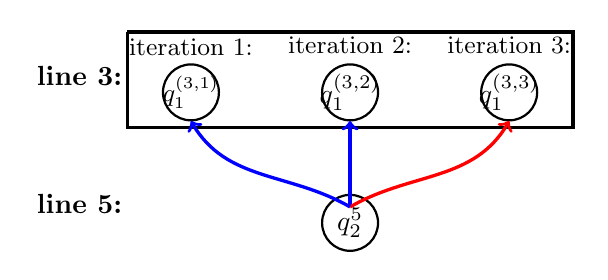
\begin{tikzpicture}[scale=\textwidth/30cm,samples=200]
%%% The nodes represents the k query in the first round
\draw[very thick] (-1,6)  -- (13,6) -- (13,3) -- (-1,3) -- (-1,6);
\draw[black] (-2.5, 4) circle (0pt) node [anchor=south]{\textbf{line 3:}};
\draw[thick] (1, 4.1) circle (25pt) 
node[label={above: \small{iteration 1:}}] {\small{$q_1^{(3,1)}$}} ;
\draw[thick] (6, 4.1) circle (25pt) node[label={[black]above: \small{iteration 2:}}] 
{$q_1^{(3,2)}$};
\draw[thick] (11, 4.1) circle (25pt) node [label={[black]above: \small{iteration 3:}}]
{$q_1^{(3,3)}$};
\filldraw[black] (-2.5, 0) circle (0pt) node [anchor=south]{\textbf{line 5:}};
\draw[thick] (6, 0) circle (25pt) node {$q_2^5$};
\draw[very thick,->, blue] (6, 0.5)  -- (6, 3.2) ;
\draw[very thick,->, red] (6, 0.5)  to [out=30,in=240] (11, 3.2) ;
\draw[very thick,->, blue] (6, 0.5)  to [out=150,in=300]  (1, 3.2) ;
\end{tikzpicture}
}
}
% \end{wrapfigure}
 \end{equation*}
 \caption{A query-based dependency graph for simplified two round algorithm}
\label{fig:simpl-two-round-graph}
\end{figure}
 %
 %
The two round algorithm consists of two main steps. The first one is asking the database through query request $q()$ for $k$ times and storing results in a list $a$. The second step is to construct another query $q_2(a)$ using the list $a$, and asks for the result from database by requesting the new query $q_2(a)$. In the loop language, the query request is assigned by $ \assign{x}{q(\expr)}$. In the above example, we simplify the query request, for example, query $q()$ in the first step does not have argument and the new constructed query is just $q(a)$ for the sake of brevity. In $TR$, we also add the line number. We do not go deep into it and
 more details about the syntax of the loop language are presented in Section~\ref{sec:loop_language}. 

% Our framework aims to provides an upper bound on the number of rounds of adaptivity (or the depth of chain of queries connected by dependency relation), denoted as $A$ in the Fig~\ref{fig:structure}, of a high level program $P$. We will go through one concrete example called "two rounds algorithm"  after the brief introduction of high level loop language, in which the target program ($TR^{H}$) implementing "two rounds algorithm" is written.

% In the high level loop language, the assignment command $x \leftarrow e$ and the loop command $\eloop ~ \aexpr  ~ \edo ~ c $ is standard. The command $ \assign{x} {q(\expr)}$ stores the result of a query $q(\expr)$ in which the elements used to construct the query are presented by the expression $\expr$. 
% We have the standard arithmatic operators denoted as $\opuls_a$, boolean operators as $\oplus_b$, and relational operators as $*_r$. 
% \[
% \begin{array}{llll}
% %  \mbox{Arithmatic Operators} & *_a & ::= & + ~|~ - ~|~ \times 
% % %
% % ~|~ \div \\  
% %   \mbox{Boolean Operators} & *_b & ::= & \lor ~|~ \land ~|~ \neg\\
% %   %
% %   \mbox{Relational Operators} & *_r & ::= & < ~|~ \leq ~|~ = \\  
% \mbox{AExpr} & \aexpr & ::= & 
% 	n ~|~ x ~|~ \aexpr *_a \aexpr ~|~ {[] ~|~ [\aexpr_0, \dots, \aexpr_i]  }  \\
% \mbox{BExpr} & \bexpr & ::= & 
% 	\etrue ~|~ \efalse  ~|~ \neg \bexpr
% 	 ~|~ \bexpr *_b \bexpr
% 	~|~ \aexpr *_r \aexpr \\
% \mbox{Command} & c & ::= &   \assign{x}{\expr} ~|~  \assign{x} {q(\expr)} ~|~  c ; c ~|~ \eif(\bexpr, c_1, c_2) 
% 	 ~|~ \eskip \sep {\eloop ~ \aexpr  ~ \edo ~ c }
% \end{array}
% \]

As shown in the left hand side of Figure~\ref{fig:structure}, our framework generates a query-based dependency graph to achieve the actual adaptivity $A$ of program $P$. This query-based dependency graph requires two main components. 
\begin{enumerate}
    \item A trace-based operational semantics to keep the history of the execution in record.
    \item A formal definition of may-dependency between two query requests.
\end{enumerate}
  % trace operation semantics
  The trace-based operational semantics of the loop language have the shape of $\config{m, c, t,w} \xrightarrow{} \config{m', c',  t', w'}  $. It works on a configuration of memory $m$, a program $c$, a trace $t$, a loop map $w$. The trace $t$ is a list of annotated queries. One annotated query is a  
  query with the annotation $(l,w)$, $l$ is the line number and $w$ is used for loop and tells the iteration number. For example, the 
  query $q()$ at line $3$ in the example $TR$ at the first iteration is represented as the annotated query $q()^{(3, [2:1])}$. The loop map $w$ is a map, from the line number of the loop counter ( $\clabel{k}^{2}$ ) to its iteration number. The trace tracks the query asked during the execution, still use the $TR$ as an example. The trace of $TR$ starting with an empty loop map $\emptyset$ has the following trace $t_{tr}$, supposing $k=3$. 
  \[t_{tr} = [q()^{(3,[2:1])},q()^{(3,[2:2])},q()^{(3,[2:3])}, q(a)^{(5,\emptyset)}  ] \]
  
% define rounds of adaptivity
The second component is the defintion of may-dependency between queries. In particular, what we need to be clear is what does it mean by saying one query may depend on another query. To this end, we look at trace.  Now whether one query $q$ depends on another query $p$ can be checked, by witnessing $q$ in the new generated trace upon change of $p$. For example, if we change the result of $q()^{(3,[2:1])}$, we have a new trace $t'_{tr}$, and $a$ may change as well. In this case, $q(a)^{(5, \emptyset)}$ may not show up in the new generated trace $t'_{tr}$. So we think $q(a)^{(5, \emptyset)}$ may depend on $q()^{(3,[2:1])}$. 
% trace based dependency relation is challenging

With the two components ready, a query-based dependency graph is built, in which the nodes are the annotated queries in the trace and the edge is the may dependency. We show a simple query-based graph below. The adpativity is obtained by finding out the longest path in the graph.
% To do, add a graph for two round
    
Now, we look at the right hand side of Figure~\ref{fig:structure}. We find the loop language is not straightforward for analysis due to the complexity of variables overwriting. 

To solve this dilemma, we transform  the program $P$ to its single static assignment(short for ssa) form $\ssa{P}$. We call it ssa language. More details about the transformation as well as the ssa language is in Section~\ref{sec:ssa}.
We briefly show our two round example in its ssa form $TR^{ssa}$ to illustrate the ssa language.
\[
TR^{ssa}(k) \triangleq
{
\begin{array}{l}
   \clabel{ a_1 \leftarrow [] }^{1}; \\
    \eloop ~ \clabel{k}^{2} ~ \edo ~ \\
    \Big(
      a_3 = \phi(a_1,a_2); \\
     \clabel{x_1 \leftarrow q() }^{3}  ; \\
    \clabel{a_2 \leftarrow x :: a_3}^{4}      \Big); \\
    \clabel{l_1 \leftarrow q(a_3)}^{5}\\
\end{array}
}
\]
We notice there is one more command without label $a_3 = \phi(a_1,a_2)$ in $TR^{ssa}$ compared to its loop variant. It adds a new variable $a_3$ whose value may come from $a_1$ or $a_2$. In the syntax of our ssa language, we use $[a_3,a_1,a_2]$ to represent this extra command in the loop command, will be discussed in Section~\ref{sec:ssa}.

Then we have our analysis algorithm $\THESYSTEM$ to directly anlayze the ssa program $\ssa{P}$ to get an upper bound. This algorithm construct a variable-based dependency graph and shows the may-dependency between annotated variables. We show the graph of our two round example.

Finally, we show that our upper bound from the variable-based dependency graph is sound with respect to our adaptivity.



% \[
%  TR^L \triangleq
% \begin{array}{l}
%     % \left[j \leftarrow 1 \right]^1 ; \\
%     \left[a \leftarrow [] \right]^1; \\
%   \eloop ~ [k]^{2} ~  
%     ~ \edo ~ \\
%   \Big( 
%      \left[x \leftarrow q \right]^3; \\
%     \left[a \leftarrow x :: a \right]^4 
%     \Big);\\
%     \clabel{
% \eswitch \Bigg(a, l, 
%     \left(\begin{array}{l}
%     \left[-n, -n, -n, \cdots, -n\right] \to q_{k + 1,1},\\
%     \cdots\\
%     \left[n, n, n, \cdots, n\right] \to q^{}_{k + 1, n^k}
% \end{array} \right) \Bigg)
%     }^5
% \end{array}
% \]
